% !TEX root = main.tex

Computational campaigns on High Performance Computing (HPC) resources can
execute compute- or data- intensive workflows and applications. On one hand,
compute-intensive applications and workflows are associated with either a single
long running executable or an ensemble of compute-intensive
tasks~\cite{balasubramanian2018harnessing}. On the other hand, data-intensive
applications are associated with multiple stages of execution which can be I/O,
memory and compute bound. While MPI is the most common programming model for
compute-intensive applications, the MapReduce~\cite{dean2004mapreduce}
abstraction is commonly used for data-intensive
applications~\cite{hellerstein2012science}.

%However, HPC resources are designed to support mainly compute-intensive long-running MPI applications, as they offer
%Not surprisingly, HPC resource architectures offer large number of computing resources, e.g., CPUs and GPUs, connected by high-end networks (e.g., Infiniband) and filesystems, such as Lustre and PVFS.
%They have however limitations in supporting data-intensive and I/O bound workflows.

Hadoop~\cite{hadoop} popularized the use of MapReduce~\cite{dean2004mapreduce}
for data-intensive applications. Hadoop's distirbuted filesystem (HDFS)
automatically partitions data and distributes them to different nodes of a
cluster machine. In addition, Hadoop's engine takes advantage of data-locality
and transfers computations to nodes, allowing to process data in parallel while
reducing data transfers. While Hadoop simplified the processing of vast volumes
of data, it has limitations in its
expressiveness~\cite{yelick2011magellan,isard2007dryad}. The complexity of
creating sophisticated applications such as, for example, iterative machine
learning algorithms~\cite{grolinger2014challenges}, required multiple MapReduce
jobs and persistence to Hadoop's Filesystem (HDFS) after each iteration. This
led to devise several higher-level abstractions and the development of
processing frameworks to implement sophisticated data pipelines.

Spark~\cite{zaharia2010spark} is the most well-known processing framework in the
Hadoop ecosystem. In contrast to MapReduce, Spark provides a richer API, more
language bindings and a memory-centric processing engine that can utilize
distributed memory and retain resources across multiple task generations.
Spark's \emph{Reliable Distributed Dataset (RDD)} ~\cite{zaharia2012resilient}
abstraction provides a powerful way to manipulate distributed collections stored
in cluster nodes' memory. Spark is used to build complex data workflows and
advanced analytic tools, such as MLLib~\cite{mllib}. Although the
addition/development of new and higher-level execution frameworks addressed some
of the problems of data processing, it introduced the problem of heterogeneity
of access and resource management.

% Problem statement.
Some computational campaigns cannot be easily classified as only compute- or
data-intensive. For example, the simulations of contemporary bio-molecular
dynamics~\cite{dror2012biomolecular} campaigns require increasing time scales
and problem sizes,  generating amounts of data several order of magnitude larger
than those so far generated. Further, data generated by those simulations often
need to be analyzed so as to determine the next set of simulation
configurations. Several tools evolved to meet the demand for molecular dynamics
data analysis, such as
MDAnalysis~\cite{michaud2011mdanalysis,gowers2016mdanalysis},
CPPTraj~\cite{roe2013ptraj} and HiMach~\cite{tiankai2008scalable}. Although
these tools offer domain-specific analytics, scaling them to high data volumes
remains a challenge, especially when the scale of the computation requires the
use of high performance computing (HPC) infrastructures. There is therefore a
need for computing environments that support scalable data processing while
preserving the ability to run simulations at large scale. To the best of our
knowledge, there does not exist a solution that provides the integrated
capabilities of Hadoop and HPC.

% Solution
In this chapter, we explore the integration between Hadoop~\cite{hadoop},
Spark~\cite{zaharia2010spark} and HPC resources. We utilize the
Pilot-Abstraction~\cite{luckow2012pstar}, allowing to manage HPC and
data-intensive applications in a uniform way. We explore two extensions to
RADICAL-Pilot~\cite{merzky2018design}, a Pilot-Job~\cite{luckow2012pstar}
runtime system designed for implementing task-parallel applications on HPC:
\begin{inparaenum}[1)]
    \item the ability to spawn and manage Hadoop/Spark clusters on HPC infrastructures on demand (Mode I); and
    \item to connect and utilize Hadoop and Spark clusters for HPC applications
    (Mode II)
\end{inparaenum}.
Both extensions facilitate the application and
resource management requirements of data-intensive applications. By supporting
these two usage modes, RADICAL-Pilot simplifies the barrier of deploying and
executing HPC and Hadoop/Spark workflows side-by-side.

The chapter is organized as follows: In section~\S\ref{sec:hpc_hadoop_rel} we
discuss the current solutions and challenges of integrating data analytics and
HPC. We continue with discussing the modes of integration and interoperability
between data analytics and HPC in~\S\ref{sec:integration_mode} and the
experimental validations of the integration in~\S\ref{sec:rph-exps}. The chapter
closes with our conclusions in section~\S\ref{sec:hpc_hadoop_concl}.


\section{Related Work and Challenges}
\label{sec:hpc_hadoop_rel}
%\subsection{Related Work}

There are several frameworks which explored the usage of Hadoop on HPC
resources, e.g., Hadoop on Demand~\cite{hod}, JUMMP~\cite{moody2013jummp},
MagPie~\cite{chu2015magpie}, MyHadoop~\cite{krishnan2011myhadoop} and
MyCray~\cite{mycray}. These frameworks provide users with a set of scripts that
can spawn and manage a Hadoop cluster on HPC resources. As soon as Hadoop is
started, users can either submit their MapReduce jobs interactively or via a
script.

Although these frameworks can spawn and manage Hadoop clusters, they isolate the
Hadoop cluster from the HPC environment. The scripts and capabilities they offer
interact directly with the HPC's submission system. As a result, users cannot
execute on the same set of nodes HPC and Hadoop applications. Further, they do
not necessarily optimize configurations and resource usage, including the use of
available SSDs, parallel filesystems and high-end network features, e.g.,
RDMA~\cite{rahman2014homr}.

%\subsection{Challenges}
Hadoop originally provided a rudimentary resource management system called the
YARN scheduler. The YARN scheduler~\cite{vavilapalli2013apache} provides an
application-level scheduling framework, addressing the increased requirements
with respect to applications and infrastructure, such as data localities
(memory, disk, datacenter), long-lived services, periodic jobs, and interactive
and batch jobs. In contrast to batch schedulers of HPC resources, YARN is
optimized for supporting data-intensive environments and managing a large number
of fine-grained tasks.

While YARN manages system-level resources, applications need to implement
application-level scheduling that optimizes their specific requirements. This is
implemented by an application-level scheduler, the \textit{Application Master},
responsible for allocating resources---called containers---and executing tasks
on these resources. In addition, Application Master manages data locality, for
example between HDFS blocks and container locations, by allocating containers on
specific nodes.

Managing resources on top of YARN poses several challenges. While applications
with fine-grained, short-running tasks are well supported, applications with
coarse-grained, long-running task, such as MPI applications, are not. To achieve
interoperability and integration between Hadoop and HPC, it is essential to
consider a more diverse set of applications on top of YARN.

A particular challenge for Hadoop on HPC deployment is the choice of storage and
filesystem backend. Typically, when using Hadoop local storage is preferred.
Nevertheless, in some cases, like when processing many small files or when
the number of parallel tasks is low to medium, random data access is required.
In those cases, using a parallel filesystem can yield a better performance. For
this purpose, many parallel filesystems provide a special client library which
improves the interoperability with Hadoop, but limits data locality and any data
placement optimization.

Another challenge is the the integration between HPC and Hadoop environments.
Rather than preserving HPC and Hadoop ``environments'' as software silos, there
is the need for an approach that integrates them. We utilize the
Pilot-Abstraction as a unifying concept to efficiently support that integration,
and not just the interoperability between HPC and Hadoop. By utilizing the
multi-level scheduling capabilities of YARN, the Pilot-Abstraction can
efficiently manage Hadoop resources, providing an application with the means to
reason about data, compute resources and allocation. In addition, we show how
the Pilot-Abstraction can be used to manage Hadoop applications on HPC
environments.

The Pilot-Abstraction~\cite{luckow2012pstar} is successfully used on HPC
resources supporting a diverse set of task-based workflows. A Pilot-job is a
placeholder job which is submitted to the resource management system and
represents a container for a dynamic set of tasks. Pilot-jobs are, also, a
well-known example of multi-level scheduling, which is often used to separate
system-level resource and user-level workload management. The Pilot-Abstraction
defines the following entities:
\begin{inparaenum} [1)]
    \item a Pilot which allocates a set of computational resources (e.g.,
    cores); and
    \item  a Compute-Unit (CU) as a self-contained piece of work represented as
    an executable.
\end{inparaenum}
The Pilot-Abstraction has been implemented within
RADICAL-Pilot~\cite{merzky2018design}.


\section{Data analytics and HPC integration: RADICAL-Pilot and YARN/Spark}
\label{sec:integration_mode}

Having established the potential of the Pilot abstraction for a range of
high-performance
applications~\cite{treikalis2016repex,ragothaman2014developing,ko2014numerical},
we use that abstraction as the starting point for integrating HPC and
data-intensive analytics. As depicted in
Figure~\ref{fig:figures_hadoop-on-hpc-viceverse}, there are at least two
different usage modes to consider:
\begin{inparaenum}[1)]
    \item Mode I: Running Hadoop/Spark applications on HPC environments (Hadoop
    on HPC),
    \item Mode II: Running HPC applications on YARN clusters (HPC on Hadoop).
\end{inparaenum}

\begin{figure}[t]
    \centering
    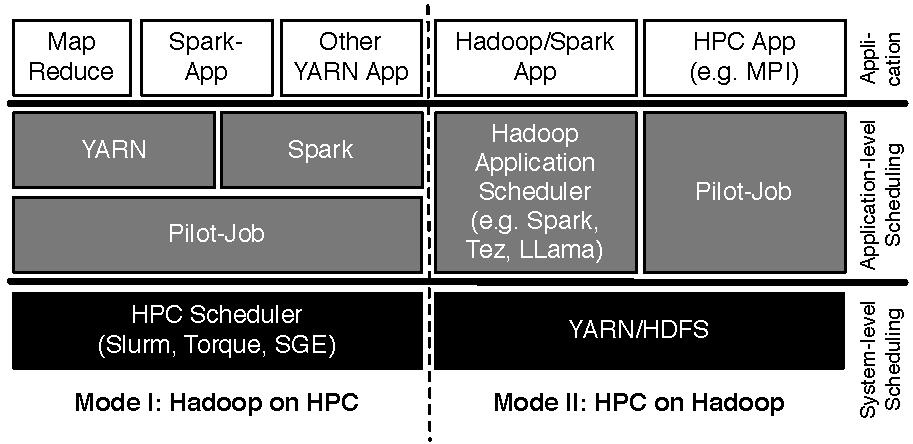
\includegraphics[width=.85\textwidth]{figures/data_analytics_hpc/hpc_hadoop/hadoop-on-hpc-viceverse.pdf}
    \caption{Hadoop and HPC Interoperability
    modes\label{fig:figures_hadoop-on-hpc-viceverse}}
\end{figure}

Mode I is critical to support traditional HPC environments so as to execute
applications with both compute and data requirements. Mode II is important for
cloud environments (e.g., Amazon's Elastic MapReduce) and an emerging class of
HPC machines with new architectures and usage modes, such as
Wrangler~\cite{wrangler}, that support Hadoop natively. For example, Wrangler
supports dedicated Hadoop environments (based on Cloudera Hadoop 5.3) via a
reservation mechanism. Using these new capabilities, applications can seamlessly
connect HPC stages (e.g., simulation stages) with analysis stages, using the
Pilot-Abstraction to provide unified resource management.

With the introduction of YARN, Hadoop can execute a broader set of applications
than before. However, developing and deploying YARN
applications, potentially side-by-side with HPC applications, remains a
difficult task. Established abstractions which are easy to use and that enable
users to reason about compute and data resources across infrastructure types
(i.e., Hadoop, HPC and clouds) are missing.

Schedulers such as YARN facilitate application-level scheduling but the
development effort required by YARN applications is still high. YARN provides a
low-level abstraction for resource management, e.g., a Java API and protocol
buffer specification. Typically, interactions between YARN and applications are
much more complex than the interactions between an application and an HPC
scheduler. Further, applications must be able to run on a dynamic set of
resources, e.g., YARN may have to preempt containers in high-load situations.
Data/compute locality requires to be manually managed by the application scheduler
by requesting resources at the location of a file chunk.
% Also, the scheduler can preempt resources (the so called YARN containers).

To address these shortcomings, various frameworks that aid the development of
YARN applications have been proposed. Llama~\cite{llama} offers a long-running
application master for YARN designed for the Impala SQL engine. Apache
Slider~\cite{apache-slider} supports long-running distributed application on
YARN with dynamic resource needs allowing applications to scale to additional
containers on demand. While these frameworks simplify development, they do not
address concerns such as interoperability and integration of HPC/Hadoop.
Integrating YARN and RADICAL-Pilot (RP) allows applications to run HPC and YARN
applications on HPC resources concurrently.

\subsubsection*{RADICAL-Pilot and YARN Overview}
\label{sssec:rp_yarn}

% RADICAL-Pilot Overview
Figure~\ref{fig:comp_rp_arch} illustrates the architecture of RP and
the components that were extended to integrate YARN. The figure on the left
shows the macro architecture of RP, while the figure on the right
shows the architecture of the RP-Agent component. RP
consists of a client module with the Pilot-Manager and Unit-Manager components
and a set of RP-Agent components running on one or more resources.
Pilot-Manager is responsible for managing a set of pilots. Pilots are described
via pilot descriptions, which contain the pilot's resource requirements.
Pilot-Manager submits a placeholder job which will run the RP-Agent
via the Resource Management System using the SAGA-API~\cite{merzky2015saga}
(steps P.1--P.2). Subsequently, the Unit-Manager and the RP-Agent
manage the execution of the application workload (the Compute-Units, steps
U.1--U.7)~\cite{merzky2019using}.

\begin{figure}
    \centering
    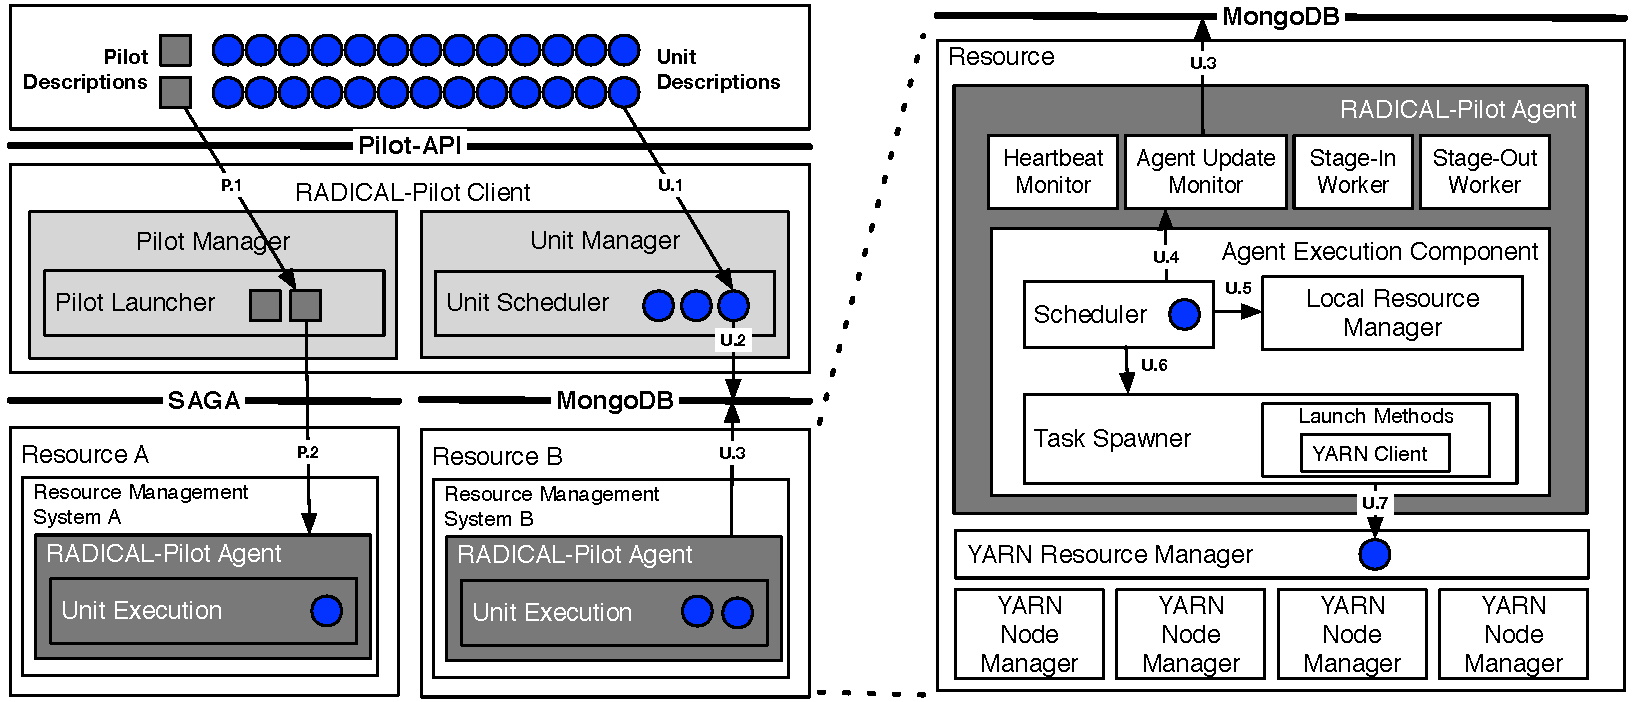
\includegraphics[width=0.85\textwidth]{figures/data_analytics_hpc/hpc_hadoop/rp-architecture-yarn.pdf}
    \caption{\textbf{RADICAL-Pilot and YARN Integration:} There are two main
    interactions between the application and RADICAL-Pilot: the management of
    Pilots (P.1--P.2) and the management of Compute Units (U.1--U.7). All YARN
    specifics are encapsulated in the RP-Agent.}
    \label{fig:comp_rp_arch}
\end{figure}

RP-Agent has a modular and extensible architecture, and consists of
the following components: Agent Execution Component, Heartbeat Monitor, Agent
Update Monitor, and Stage In and Stage Out Workers. The main integration of YARN
and RP is done in Agent Execution Component. The Agent Execution component
consist of four sub-components:
\begin{inparaenum}[a)]
    \item the \textit{scheduler} is responsible for monitoring the resource
    usage and assigning CPUs/GPUs to CUs;
    \item the \textit{Local Resource Manager} (LRM) interacts with the batch
    system and communicates to the pilot the available number of computing
    resources and how they are distributed;
    \item the \textit{Task Spawner/ Executor} configures the execution
    environment, executes and monitors each unit; and
    \item the \textit{Launch Method} encapsulates the environment specifics for
    executing an application, e.g., the usage of \texttt{mpiexec} for MPI
    applications, machine-specific launch methods (e.g. \texttt{aprun} on Cray
    machines) or the usage of YARN.
\end{inparaenum}
After a unit completes its execution, the Task Spawner collects the exit code,
standard output, and informs the scheduler about the freed cores.

\subsubsection*{RADICAL-Pilot and YARN Integration}
\label{sssec:rp-yarn}

There are two main approaches to the integration of RP and YARN: (i)
Integration at the Pilot-Manager level via a SAGA adaptor; and (ii) integration
at the RP-Agent level. The first approach poses several challenges,
among which the most difficult to address is that, typically, firewalls prevent
the communication between external machines and a YARN cluster. A YARN
application is not only required to communicate with the resource manager, but
also with the node managers and containers. Further, this approach would require
significant extension of Pilot-Manager, which currently relies on the SAGA Job
API for launching and managing pilots. Capabilities required by YARN, like
on-demand provisioning of a YARN cluster and application resource management,
are very difficult to implement via the SAGA API.

The second approach encapsulates YARN specifics at resource-level, enabling the
decentralized provision of a YARN cluster. Units are scheduled and submitted to
the YARN cluster via the Unit-Manager and RP-Agent scheduler. By
integrating RP and YARN at the RP-Agent level, RP can support both Mode I
and II, as outlined in Figure~\ref{fig:figures_hadoop-on-hpc-viceverse}.

As illustrated in Figure~\ref{fig:comp_rp_arch}, RP (steps P.1--P.2)
starts on the remote resource using SAGA. In Mode I, during the launch of
RP-Agent a YARN cluster is spawned on the allocated resources (Hadoop
on HPC), while in Mode II, RP-Agent connects to a YARN cluster that
runs on the resources managed by RP-Agent. Once started, RP-Agent
 accepts CUs submitted via Unit-Manager (step U.1).
Unit-Manager queues new CUs using a shared MongoDB (step U.2)
database. RP-Agent periodically checks for new CUs (step
U.3) and queues them in the scheduler (step U.4). Finally, the Executor manages
the execution of the CUs (step U.6 and U.7).

The \emph{Local Resource Manager (LRM)} provides an abstraction to local
resource details for other components of the RP-Agent. The LRM
evaluates the environment variables provided by the resource management systems
to obtain information, such as the number of cores per node, memory and the
assigned nodes. This information can be accessed through the Resource Manager's
API. In Mode I (Hadoop on HPC), during the initialization of the
RP-Agent, the LRM setups the HDFS and YARN daemons. First, the LRM
downloads Hadoop and creates the necessary configuration files, i.e., the
\texttt{mapred-site.xml}, \texttt{core-site.xml}, \texttt{hdfs-site.xml},
\texttt{yarn-site.xml} and the slaves and master file containing the allocated
nodes. The node that is running the Agent, runs the master daemons of Hadoop:
the HDFS Namenode and the YARN Resource Manager.
As soon as HDFS and YARN area active, the scheduler receives meta-data about
the cluster, i.e., the number of cores and memory. HDFS and YARN remain
active until all tasks are executed. Before termination of the agent, the
LRM stops the Hadoop and YARN daemons and removes the associated data files. In
Mode II (Hadoop on HPC), the LRM solely collects the Hadoop cluster resource
information.

The \emph{scheduler} is another extensible component of the RP-Agent
responsible for queuing CUs and assigning them to resources. To
support YARN, we created a special scheduler that utilizes the cluster state
information (e.g., the amount of available cores, memory, queue information,
application quotas etc.) obtained via the Resource Manager's REST API of YARN.
In contrast to other RP schedulers, our scheduler specifically
utilizes memory in addition to cores for assigning resources to CUs.

The \emph{Task Spawner} is responsible for managing and monitoring the execution
of a CU. The \emph{Launch Method} component encapsulates
resource/launch-method specific operations, e.g., the usage of the \texttt{yarn}
command line tool for submitting and monitoring applications. After the launch
of a CU, Task Spawner periodically monitors its execution and updates
its state in a shared MongoDB instance by utilizing the application log file.

\begin{figure}[t]
    \centering
    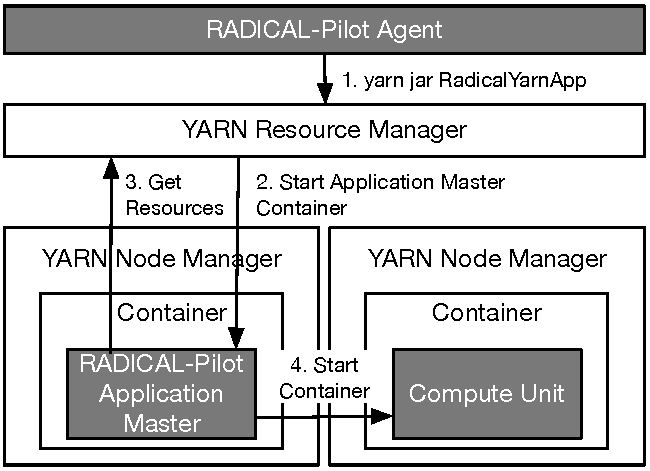
\includegraphics[width=.65\textwidth]{figures/data_analytics_hpc/hpc_hadoop/yarn.pdf}
    \caption{RADICAL-Pilot YARN Agent Application.}
    \label{fig:figures_yarn}
\end{figure}

\emph{RADICAL-Pilot Application Master:} YARN's multi-step resource allocation
process depicted in Figure~\ref{fig:figures_yarn} differs significantly from HPC
schedulers and, as such, poses an integration challenge. The central component
of a YARN application is the Application Master, which negotiates resources
assignment with the YARN Resource Manager and manages the execution of an
application in the assigned resources. The unit of allocation in YARN is a
container~\cite{murthy2014apache} (not to be confused with a Docker container).
The YARN client is part of the YARN Launch Method and implements a YARN
Application Master, which is the central instance for managing the resource
requirements of an application. RP utilizes a managed application
master that runs inside a YARN container. Once the Application Master container
is started, the managed application master requests a YARN container that meets
the resource requirements of the CU from the YARN's Resource Manager.
Once YARN allocates a container, the CU starts inside that container. A wrapper
script sets up a RP environment, staging the specified files and
running the executable defined in the CU Description. Every Compute
Unit is mapped to a YARN application consisting of an Application Master and a
container of the size specified in the CU Description.

\subsubsection*{RADICAL-Pilot and Spark Integration}
\label{sssec:rp_spark}

Spark offers multiple deployment modes: standalone, YARN and Mesos. While it is
possible to support Spark on top of YARN, the YARN and Mesos approaches incur
into significant complexities and overheads as they require for two frameworks
to be configured and bootstrapped. Since RP operates in user-space
and single-user mode, no advantages with respect to using a multi-tenant YARN
cluster environment exist. Thus, we support Spark via the standalone deployment
mode.

Similar to the YARN integration, the necessary changes for Spark are confined to
the RP-Agent. Local Resource Manager (LRM) initializes and deploys
the Apache Spark environment. In the first step, LRM detects the number of
cores, memory and nodes provided by Resource Management System, and verifies and
downloads necessary dependencies (e.g., Java, Scala, and Spark binaries). In the
second step, LRM creates the necessary configuration files to run a multi-node,
standalone Spark cluster (e.g., \texttt{spark-env.sh}, \texttt{slaves} and
\texttt{master} files). Finally, LRM starts a Spark cluster, using the
previously generated configuration.

Similar to YARN, a Spark RP-Agent scheduler is used
for managing Spark resource slots and assigning CUs. During the termination of
the RP-Agent, LRM shuts down the Spark cluster using
Spark’s termination script, which stops both the master and the slave nodes.
Similarly, the Spark specific methods for launching and managing CUs
on Spark are encapsulated in a Task Spawner and Launch Method component.

\section{Experiments and Evaluation}
\label{sec:rph-exps}

To evaluate the RADICAL-Pilot-YARN (RP-YARN) and Spark extension, we conduct two
experiments. In \S\ref{ssec:startup_pilot_unit}, we analyze and compare
RP and RP-YARN with respect to startup times of both the
Pilot and the CUs. In \S\ref{ssec:kmeans}, we use the well-known
K-Means algorithm to investigate the performance and runtime trade-offs of a
typical data-intensive application. We performed our experiments on two XSEDE
machines: Wrangler~\cite{wrangler} and Stampede~\cite{stampede}. On Stampede,
every node has 16 cores and 32 GB of memory; on Wrangler 48 cores and 128 GB of
memory. For our experiments, we used RP v0.45, Hadoop v2.6 and Spark
v2.0.2.

\subsection{Pilot Startup and Compute Unit Submission Characterization}
\label{ssec:startup_pilot_unit}

\begin{figure}[t]
    \centering
    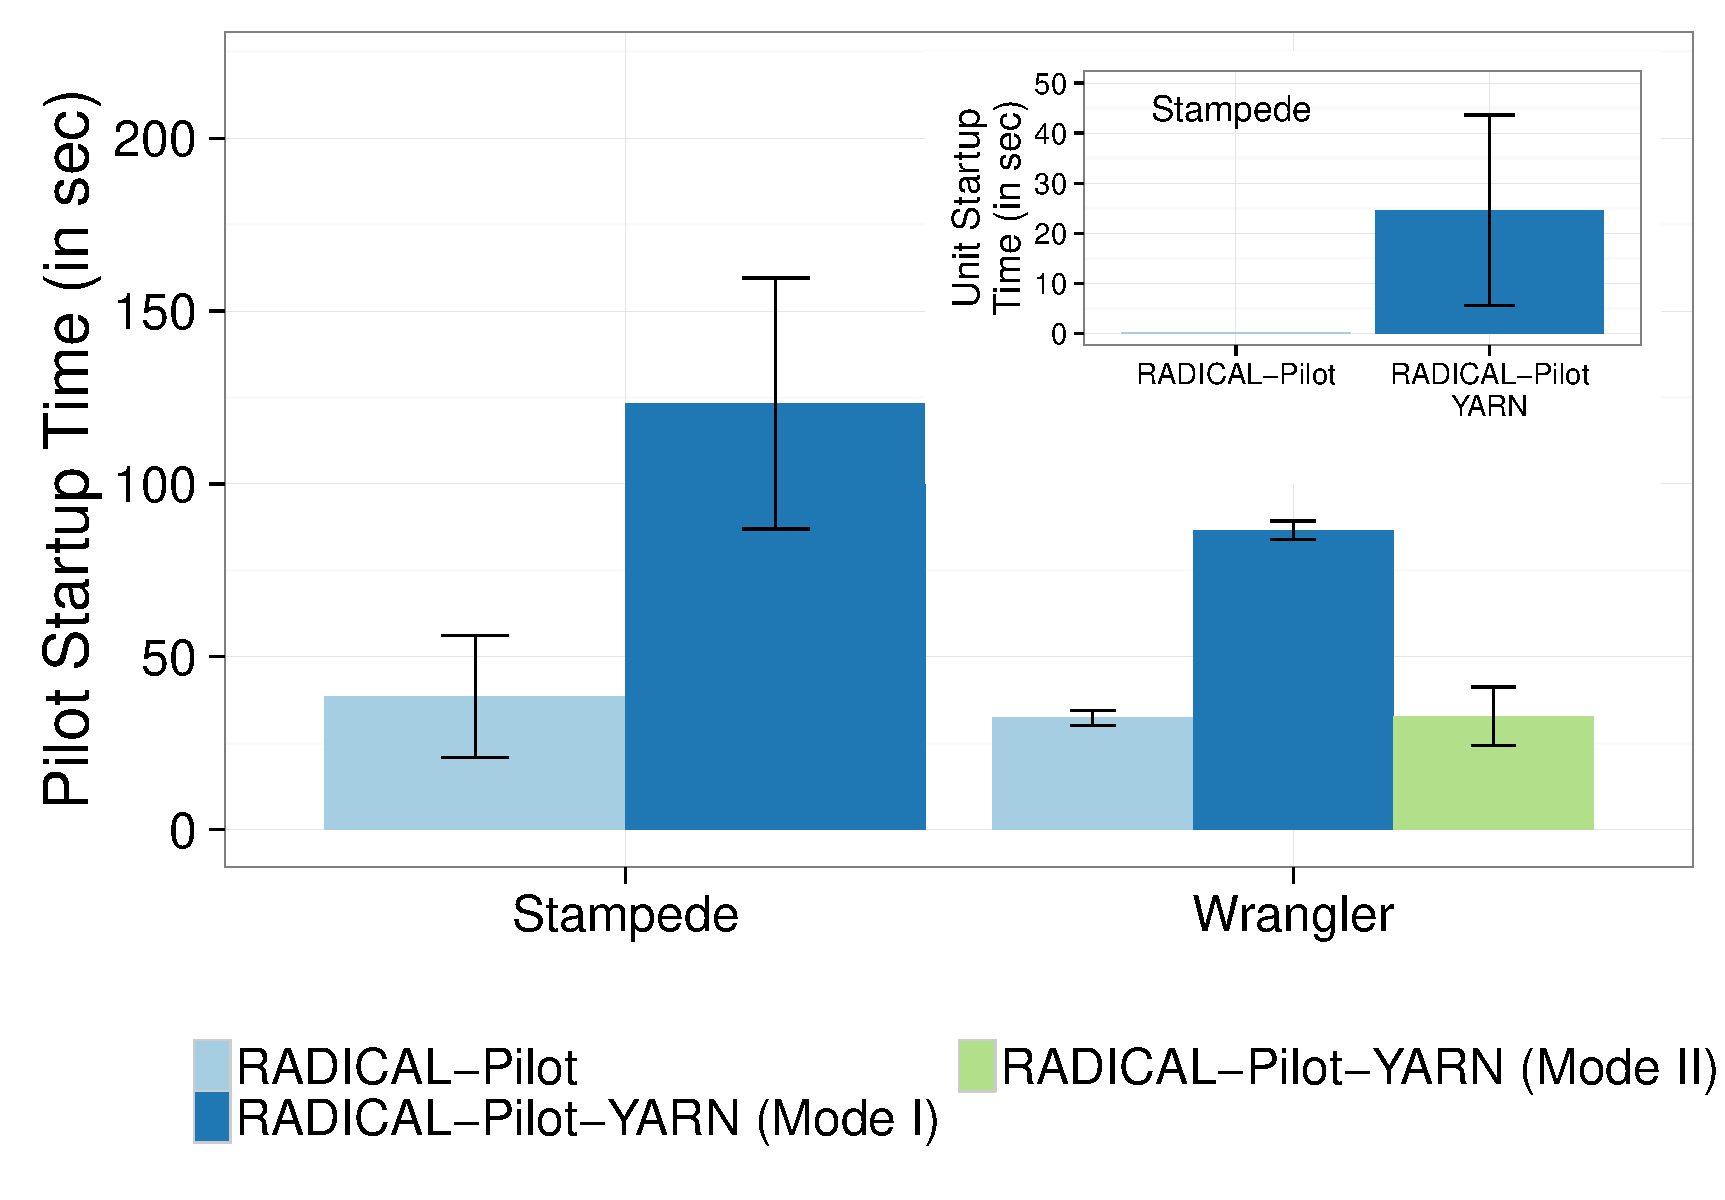
\includegraphics[width=0.75\textwidth]{figures/data_analytics_hpc/hpc_hadoop/pilot_unit_startup.pdf}
    \caption{RADICAL-Pilot and RADICAL-Pilot-YARN startup overheads.
        \label{fig:startup_yarn}}
\end{figure}

In Figure~\ref{fig:startup_yarn} we analyze the measured overheads when starting
RP and RP-YARN, and when submitting CUs. The
agent startup time for RP-YARN is defined as the time between when
RP-Agent starts and when the first CU starts executing. On
Wrangler, we compare both Mode I (Hadoop on HPC) and Mode II (HPC on Hadoop).
For Mode I, the startup time is higher compared to the startup time of
RP and of Mode II. This can be explained by the necessary steps
required to download, configure and start the YARN cluster. For a single node
YARN environment, the overhead for Mode I (Hadoop on HPC) is between 50-85\,sec,
depending on the selected resource. The startup times for Mode II on
Wrangler---using the dedicated Hadoop environment provided via the data
portal---are comparable to the normal RP startup times as RP does not
spawn a Hadoop cluster.

The inset of Figure~\ref{fig:startup_yarn} shows the time taken to start Compute
Units via RP to a YARN cluster. For each CU, resources have to be
requested in two stages: first the application master container is allocated
and, second, the containers for the actual compute tasks becomes available. For
short-running jobs, that represents a bottleneck. In summary, while there are
overheads associated with executing CUs inside of YARN, we believe
these are acceptable, in particular for long-running CUs.
%The novel capabilities of executing HPC tasks and YARN tasks
%within the same application has significant benefits for which the overheads we
%measured are likely acceptable. \mtnote{why?}

\subsection{K-Means Performance Characterization}
\label{ssec:kmeans}

We compare the time to completion of the K-Means algorithm using two
configurations: RP on HPC and RP in HPC/YARN mode. We use
three different scenarios: 10,000 points and 5,000 clusters, 100,000 points and
500 clusters, and 1,000,000 points and 50 clusters. Each point belongs to a
three dimensional space. The compute requirements depend on the product of the
number of points and clusters, thus the requirements are constant for all three scenarios. We
use an optimized version of K-Means in which the sum and number of points are
precomputed in the map phase, thus only these two attributes per cluster need to
be shuffled. The shuffle traffic depends on the number of clusters and decreases
with the number of clusters. For the purpose of this benchmark, we run two
iterations of K-Means.

We utilize up to 3 nodes on Stampede and Wrangler. We use the following
configurations for our experiments: 8 tasks on 1 node, 16 tasks on 2 nodes and 32
tasks on 3 nodes. For RP-YARN, we use Mode II (Hadoop on HPC): the
YARN Resource Manager is deployed on the node running the RP-Agent.

Figure~\ref{fig:experiments_kmeans_rpyarnkmeans} shows the results of executing
K-Means over different scenarios and configurations. For RP-YARN,
runtimes include the time required to download and start the YARN cluster on the
allocated resources.

\begin{figure}[t]
    \centering
    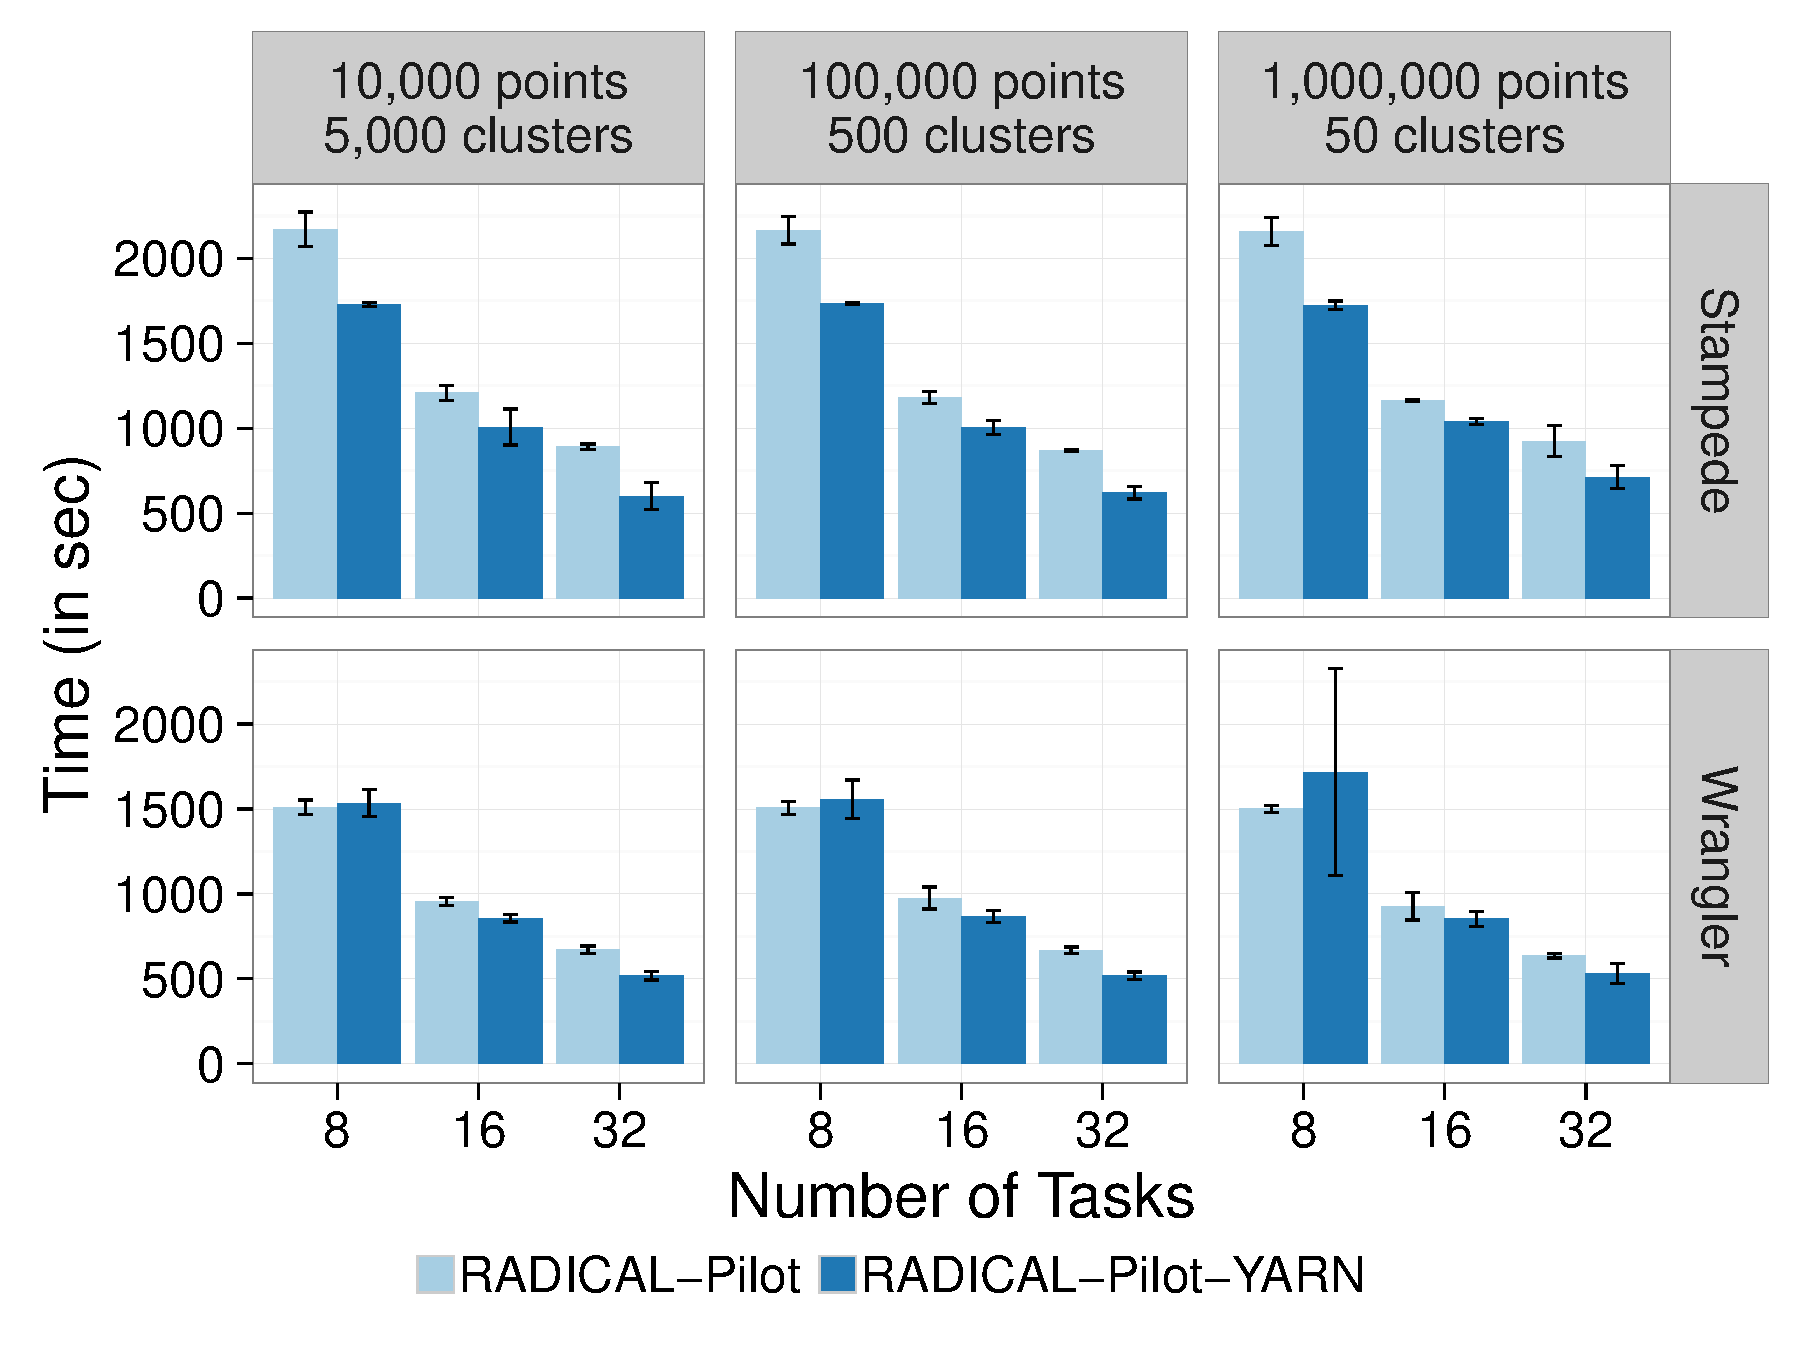
\includegraphics[width=.75\textwidth]{figures/data_analytics_hpc/hpc_hadoop/kmeans.pdf}
    \caption{RADICAL-Pilot and YARN-based K-Means time to completion on Stampede and Wrangler.}
    \label{fig:experiments_kmeans_rpyarnkmeans}
\end{figure}

Independent of the scenario, runtimes decrease with the number of tasks. In
particular, for the 8 task scenarios the overhead of YARN on Wrangler is
enough to produce higher runtimes for RP-YARN than RP. For larger number of
tasks, we observed on average 13~\% shorter runtimes for RP-YARN.
Also, RP-YARN achieves better speedups, e.g., 3.2 for 32 tasks for
the 1 million points scenario, which is significantly higher than the
RP speedup of 2.4 (both on Wrangler and compared to base case of 8
tasks). One of the reasons of that performance difference, is that
RP-YARN uses the local file system, while RP uses the
Lustre filesystem.

For similar scenarios and task/resource configuration, the runtimes show a
significant performance improvement on Wrangler over Stampede. This is
attributed to the better hardware (CPUs, memory) of Wrangler than Stampede. In
particular, for RP-YARN we observed on average higher speedups on
Wrangler, indicating that we saturated the 32 GB of memory available on each
Stampede node.

In summary, despite the overheads of RP-YARN with respect to Pilot
and CU startup time, we were able to observe performance improvements
(on average 13~\% better time to completion than RP) mainly due to
the better performance of the local disks.


\section{Conclusions}
\label{sec:hpc_hadoop_concl}

An increasing number of scientific applications use Hadoop and Spark mainly due
to the accessible abstractions they provide. HPC and Hadoop environments are
converging: For example, MLLib/Spark utilize BLAS, and Hadoop frameworks adopt
parallel and in-memory computing concepts that originated in HPC. Currently,
traditional HPC applications lack the ability to use Hadoop and other Hadoop
tools, without sacrificing the advantages of HPC environments. One prominent
reason for the limited uptake of Hadoop-based technologies on HPC
infrastructures is the lack of effective, scalable and usable resource
management techniques.

This chapter shows how the Pilot abstraction can be used as an integrating
concept, discussing the design and implementation of RP extensions
for Hadoop and Spark, and validating those extensions with scalability analysis
on two HPC infrastructures. The Pilot abstraction enables users to combine the
capabilities of best-of-breed tools which run on heterogeneous HPC
infrastructures. Using these capabilities, data-intensive computational
campaigns can utilize diverse Hadoop and HPC frameworks, enabling
scalable data workflows and analytics pipelines.

In this chapter we demonstrated the importance of integrated capabilities for
supporting data-intensive workflows on HPC infrastructures. In the next chapter,
we move forward by characterizing the performance of those capabilities for
paradigmatic molecular dynamics workflows. When executing computational
campaigns on HPC resources is paramount to understand the performance tradeoffs
among application, middleware, executable and system capabilities.

%%%%%%%%%%%%%%%%%%%%%%%%%%%%%%%%%%%%%%%%%%%%%%%%%%%%%%%%%%%%%%%%%%%%%%%%%%%%%%%%
%
%For example, Cray's analytics platform Urika~\footnote{http://www.cray.com/products/analytics} has Hadoop and Spark running on HPC architecture as opposed to regular clusters, but without the HPC software environment and capabilities.
%However, several applications ranging from bio-molecular simulations to epidemiology models~\cite{network1} require significant simulations interwoven with analysis capabilities such as clustering and graph analytics; in other words some stages (or parts of the same stage) of an application would ideally utilize Hadoop/Spark environments and other stages (or parts thereof) utilize HPC environments.
%
%Over the past decades, the High Performance Distributed Computing (HPDC) community has made significant advances in addressing resource and workload management on heterogeneous resources.
%For example, the concept of multi-level scheduling~\cite{1392910} as manifested in the decoupling of workload assignment from resource management using the concept of intermediate container jobs (also referred to as \pilotjobs~\cite{pstar12}) has been adopted for both HPC and Hadoop.
%Multi-level scheduling is a critical capability for data-intensive applications as often only application-level schedulers can be aware of the localities of the data sources used by a specific application.
%This motivated the extension of the \pilot-Abstraction to \pilotdata~\cite{pilot-data-jpdc-2014} to form the central component of a resource management middleware.
%
%In the following sections, we discuss a set of tools for supporting both of these usage modes:
%In section~\ref{ssec:saga_hadoop} we present SAGA-Hadoop, a light-weight tool for running Hadoop on HPC (Mode I).
%We then discuss, the integration of Hadoop and Spark runtimes into Compute Unit, which enables both the interoperable use of HPC and Hadoop, as well as the integration of HPC and Hadoop applications (Mode I and II) (Section~\ref{ssec:rp-impl}).
%Using these new capabilities, applications can seamlessly connect HPC stages (e.g., simulation stages) with analysis staging using the Pilot-Abstraction to provide unified resource management.
%
%\subsection{Mode I: SAGA-Hadoop, supporting Hadoop/Spark on HPC}
%\label{ssec:saga_hadoop}
%
%SAGA-Hadoop~\cite{saga-hadoop} is a tool for supporting the deployment of Hadoop and Spark on HPC resources (Mode I in Figure~\ref{fig:figures_hadoop-on-hpc-viceverse}).
%Using SAGA-Hadoop an applications written for YARN (e.g., MapReduce) or Spark (e.\,g. PySpark, DataFrame and MLlib applications) can be executed on HPC resources.
%
%Figure~\ref{fig:saga-hadoop} illustrates the architecture of SAGA-Hadoop.
%SAGA-Hadoop uses SAGA~\cite{merzky2015saga} to spawn and control Hadoop clusters inside an environment managed by an HPC scheduler.
%SAGA is used for dispatching a bootstrap process that generates the necessary configuration files and starting Hadoop.
%The specifics of the Hadoop framework (i.e., YARN and Spark) are encapsulated in a Hadoop framework plugin (also referred to as adaptors).
%SAGA-Hadoop delegates tasks, such as the download, configuration and start of a framework to this plugin.
%In the case of YARN, the plugin is then responsible for launching YARN's Resource and Node Manager processes; in the case of Spark, the Master and Worker processes.
%This architecture is extensible as new frameworks, e.g., Flink, can easily be added.
%
%\begin{figure}[t]
%    \centering
%    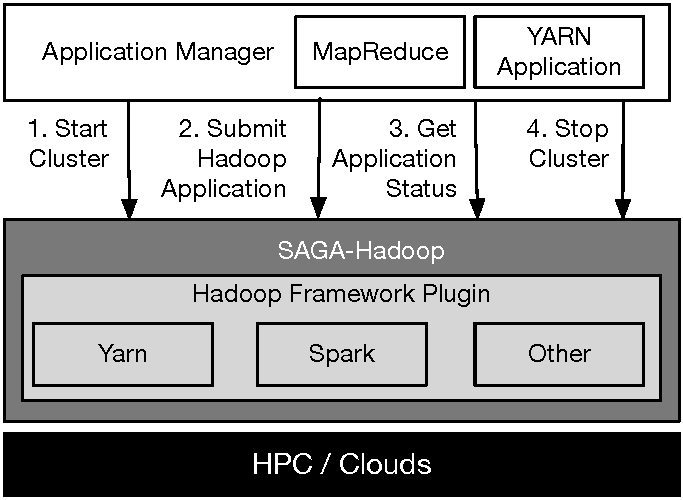
\includegraphics[width=.95\textwidth]{figures/data_analytics_hpc/hpc_hadoop/pilot-abds.pdf}
%    \caption{SAGA-Hadoop for HPC and Cloud Infrastructures.}
%    \label{fig:saga-hadoop}
%\end{figure}
%
%While nearly all Hadoop frameworks (e.g., MapReduce and Spark) support YARN for resource management, Spark provides a standalone cluster mode, which is more efficient in particular on dedicated resources.
%Thus, a special adaptor for Spark is provided.
%Once the cluster is setup, users can submit applications using SAGA's API that allows them to start and manage YARN or Spark application processes.
%
%While SAGA-Hadoop provides the interoperability between YARN and HPC resources by treating YARN as a substitute for common HPC schedulers, the integration of YARN and HPC applications or application stages remains challenging.
%As a consequence, we explored the usage of the Pilot~-Abstraction~\cite{luckow2012pstar}, through RADICAL-Pilot~\cite{merzky2019using}, to enable the integration between these different application types.